\chapter{Mathoden und Techniken}
    \begin{itemize}
        \item Wozu UHV
        \item Oberflächensensetive Methoden
    \end{itemize}
\section{LEED}
    \begin{itemize}
        \item Geometrische Struktur
        \item Mathematische Methoden
    \end{itemize}
\section{PES}
    \begin{itemize}
        \item XPS
        \item UPS
        \item Modele der Anregung
        \item Mittlere Frei weglänge
        \item Integrierte Spektren
    \end{itemize}

\section{ARPES}
    \begin{itemize}
        \item 
    \end{itemize}

    \section{Moment Mikroskopie} \label{sec:MM}
        Bei der Moment Microskopie (\textit{engl.} Momentum Microscopy) ist eine sehr viel versprechende Technik, die für immer mehr Aufsehen in den letzten Jahren gesorgt hat.
        Der größte Vorteil liegt wohl in der Kombination von spektroskopischen Methoden und mikroskopischen Methoden.
        Zuerst wurde dies 1933 durch E. Brüche entdeckt, der eine Zinkplatte mit Hilfe von Photoelektronen und einer magnetischen Linse auf einem Leuchtschirm abbildete \cite{bruche_elektronenmikroskopische_1933}.

        Bei der Moment Mikroskopie ist die zeitgleich Erfassung des polaren und azimuntalen Austrittswinkel von großer Bedeutung. 
        Zusätzlich werden die Elektronen auch nach ihrer kinetsichen Energie sortiert, sodass ein dreidimensionaler Datensatz entsteht.

        \begin{figure}
            \centering
            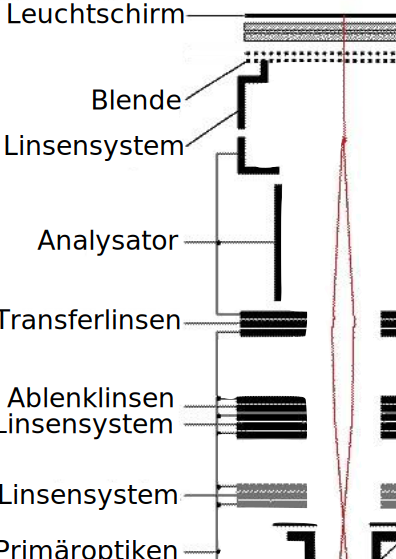
\includegraphics[width=0.7\textwidth]{./content/PEEM_schemaneu.jpg}
            \caption{Exemplarischer Aufbau eines Momentum Microskope. Aus \cite{KUCH}.}
            \label{fig:MM}
        \end{figure}
        Ein exemplarischer Aufbau ist in Abbildung \ref{fig:MM} zu sehen.
        Die durch die Photonen angeregten Elektronen werden durch ein starkes elektrisches Feld von einigen \si{\kilo\volt} von der Probe zum Analysator hin beschleunigt.
        Das Extractorfeld kann bis auf \SI{29}{\kilo\volt} erhöht werden, wird standardmäßig aber auf \SI{10}{\kilo\volt} festgesetzt
        Durch diese große Spannung zwischen Probe und Extraktor ist es möglich ein ein großen Sichtbereich im Impulsraum abzudecken.
        Dies ist nötig, da durch den streifenden Einfall der Photonen und der Abberation der elektrostatischen Linsen nur einen kleinen Akzeptanzwinkel zur Verfügung stehen würde. \textbf{QUELLE}
        Wichtig bei der Kathoden Linse ist, dass das Feld zwischen Probe und Linse sehr homogen ist, damit der Austrittswinkel erhalten bleibt.
        Anschließend werden die Elektronen durch elektrostatische Linsen fokusiert und durch die einzelnen Blenden geleitet.
        Sie sind so konzipiert, dass die Bildebene und die hintere Brennebene immer an der selben Position, der Blenden bleiben.
        Mit Hilfe von Kontrastblenden kann dann eine Auflößung von einigen \si{\nano\meter} erreicht werden. \textbf{QUELLE}.
        Hierbei gibt es an zwei verschiedenen Stellen Blenden, je nach dem ob im Realraum oder im Impulsraum ein Bild aufgenommen werden soll.
        Damit der Spot auch immer im Zentrum der Blenden liegt gibt es im Linsensystem noch elektrostatische Verschiebungslinsen, welche den Strahl ablenken.
        Nach den Blenden folgt ein weiters Linsensystem aus elektrostatischen Linsen, welche das Bild auf den Ausgang des Linsensystems fokussieren.
        Hier befinden sich zwei magnetische Verschiebungslinsen um Drift zu korrigieren.
        Im Anschluss gehen die Elektronen in ein Transferlinsensystem über, welches dafür sorgt, dass ein einszueins Abbild auf die Eingagnsblende das Analysators trifft.
        Die Eingagnsblende kann in ihrer Größe varriert werden, sodass nur ein Teil der Elektronen in den Analysator eintreten.
        Je kleiner die Blende gewählt wird, desto besser ist die Energieauflösung aber so kleiner die Gesamtintensität.
        Im Analysator selbst unterliegen die Elektronen der energieabhängigen Dispersion im elektrischen Feld. 
        Nur Elektronen mit der passenden Energie verlassen den Analysator durch die Ausgangsblende.
        Nach dem Detektor gibt es eine weiter Linseneinheit, welche zusammen mit einer Blende das gewünschte energieaufgelöst Bild auswählt und es auf die Detektorgröße aufweitet.
        Anschließend durchlaufen die Elektronen eine Mikrokanalplate (eine Art Elektronenvervielfacher) und prallen auf den Phosphorschirm, der an den entsprechenden Stellen aufleuchtet.
        Durch die Kamera wird diese Leuchten regestriert und das räumliche oder rekrusives Bild kann rekostruiert werden \cite{SPECS-MM}.

        \subsection{Impulsraum Aufnahmen}
        Bei der Aufnahme im Impulsraum wird bei der gesamten Abbildungsoptik der Austrittswinkel erhalten.
        Das verwendete Mikroskop kann einen Austrittswinkel von biszu $\pm\SI{90}{\degree}$ erfassen für eine Energie kleiner als \SI{50}{\electronvolt} \cite[page=21]{SPECS-MM}.
        Für größere kinetische Energien wird das Sichtfeld auf $\pm\SI{3.6}{\angstrom}$ beschränkt.
        Dabei spielt es keine Rolle wo auf der Probe die Elektronen emittiert werden.

        Um ein Bild im Impulsraum aufzunehmen wird die Blende im der Bildebene eingefahren, die so genannte Feldblende (\textit{field aperture}).
        Durch die Blende wird ein Ausschnitt auf der Probe ausgwählt, von der die emittierten Elektronen erfasst werden.
        Bei einem Blendendurchmesser von \SI{20}{\micro\meter} und der Standard-Vergrößerung von \num{5} ist der ausgewählt Bereich etwa \SI{4}{\micro\meter} groß.

        \subsection{realraum Aufnahmen}
        Es ist ferner möglich Bilder im Realraum aufzunehmen. 
        Dabei können sehr kleine Spots von \SIrange[range-pharse=' bis ']{50}{200}{\micro\meter} ausgewählt werden.
        Das Bild wird dann bei festen Energiefilter-Einstellungen aufgenommen.

        Um den Kontrast im Bild zu erhöhen werden nur Elektronen mit einem bestimmten Austrittswinkel für die Erstellung des Bildes erfasst.
        Dies geschieht durch Einsetzen einer Blende in dem hinteren Brennpunkt, die Kontrastblende (\textit{contrast aperture}).



        \begin{figure}
            \centering
            \includegraphics[width=0.7\textwidth]{./content/Real_k.PNG}
            \caption{Die verschiedenen Konfiguration der Blenden um zwischen Realraum Bild und Impulsraum Bild umzuschalten. Aus \cite{Focus}.}
            \label{fig:real_k}
        \end{figure}
        Für den Impulsraum ist dies in Abbildung \ref{fig:real_k}\,a und für den Realraum in Abbildung \ref{fig:real_k}\,b dargestellt.
        Um ein Bild im Realraum zu erhalten muss die Blende im Brennpunkt eingesetzt sein, auf dem Eintrittsspalt des Energyanalysators wird dann das Bild der Oberfläche projeziert.
        Wird hingegen in der ersten Bildebene die Blende eingesetzt so wird auf dem Eintrittsspalt das Beugungsbild abgebildet. 
        Die restlichen Linsen, Stigmatoren und Ablenker sind dafür da, dass Bild zu zentrieren und Abberation auszugleichen.

        Als Energiealysator kommt ein hemisphärischer Analysator zum Einsatz, für gepulste Photonenquellen würde sich auch ein \textit{Time of flight - TOF} (Flugzeit) Analysator eignen.
        Bei dem hemisphärischer Analysator werden die Elektronen zwischen zwei Halbkugeln durch ein statisches elektrisch Feld auf eine Kreisbahn gezwungne.
        Dabei ist das Feld so gewählt, dass nur die mit der richtigen kinetischen Energie eintretenden Elektronen auch auf den Austrittsspalt abgebildet werden.
        Bei einem TOF Analysators wird die kinetische Energie aus der Flugzeit der Elektronen bestimmt, weswegen es nur für gepulste Photonenquellen möglich ist.

        Nach dem Energiealysator gibt es nochmal ein paar Optiken, die das Bild auf den Detektor abbilden.
        Bei dem Detektor handelt es sich um eine CMOS Kamera die das Bild der auf den Leuchtschirm auftreffenden Elektronen aufnimmt.
        Der Vorteil der CMOS (\textit{Complemantary metal-oxid-semiconductor}) Kamera Technik gegnüber der klassischen CCD (\textit{Charge Coupled Device}) Kamera Technik ist, dass erlaubt es wahre Pulszählraten zu erfassen 
        Dabei wird ein einzelnes Bild in nur wenigen Millisekunden erfasst, dies ist durch die Kombination von Kamera und Grafigprozessor möglich.
        Die CCD Detektoren sind ein Standard bei ARPES Messungen, sie integrieren die analoge Photonenintensitäten oder einzelne Lichtblize werden aufgezeichnet.
        Einer der Nachteile ist die geringe Abtastrate auf Grund der hohen Erholungszeit.

        \cite{CMOS}.

      
        \begin{figure}
            \centering
            \includegraphics[width=0.7\textwidth]{./content/MM.png}
            \caption{Der für die durchgeführten Experimente verwendete Aufbau.}
            \label{fig:aufbau}
        \end{figure}
        Der gesamte Aufbau aus dem PEEM und der Präperationskammer ist in Abbildung \ref{fig:aufbau} zu finden.

        \begin{itemize}
            \item Erweiterung auf Spinaufgelöst möglich
            \item TOF
            \item Zeitaufgelöst
            \item Real und Impulsraum
        \end{itemize}

    \section{Molekül Orbital Tomographie}
        Die Molekühle Orbital Tomographie vereinigt nun die Vorteile des Momentum Mikroskopes mit der Theorie der Dichtefunktionaltheorie (DFT) um Molekühlorbitale zu identifizieren.
        \begin{itemize}
            \item Vereinigung von Experiment und Theorie
            \item MM
        \end{itemize}

